\documentclass[10pt,aspectratio=169]{beamer}
\usetheme{Madrid}
\usepackage[utf8]{inputenc}
\usepackage[russian]{babel}
\usepackage{amsmath,amsfonts,amssymb}
\usepackage{tikz}
\usetikzlibrary{positioning,arrows,shapes}

\title{Dots and Boxes Assistant}
\subtitle{Администрирование игры «Палочки»}
\author{Парфёнова Виктория Вадимовна, 25.Б42-мм}
\date{23.05.2026}

\begin{document}

\begin{frame}
\titlepage
\end{frame}

\begin{frame}{Правила игры}
\begin{center}
    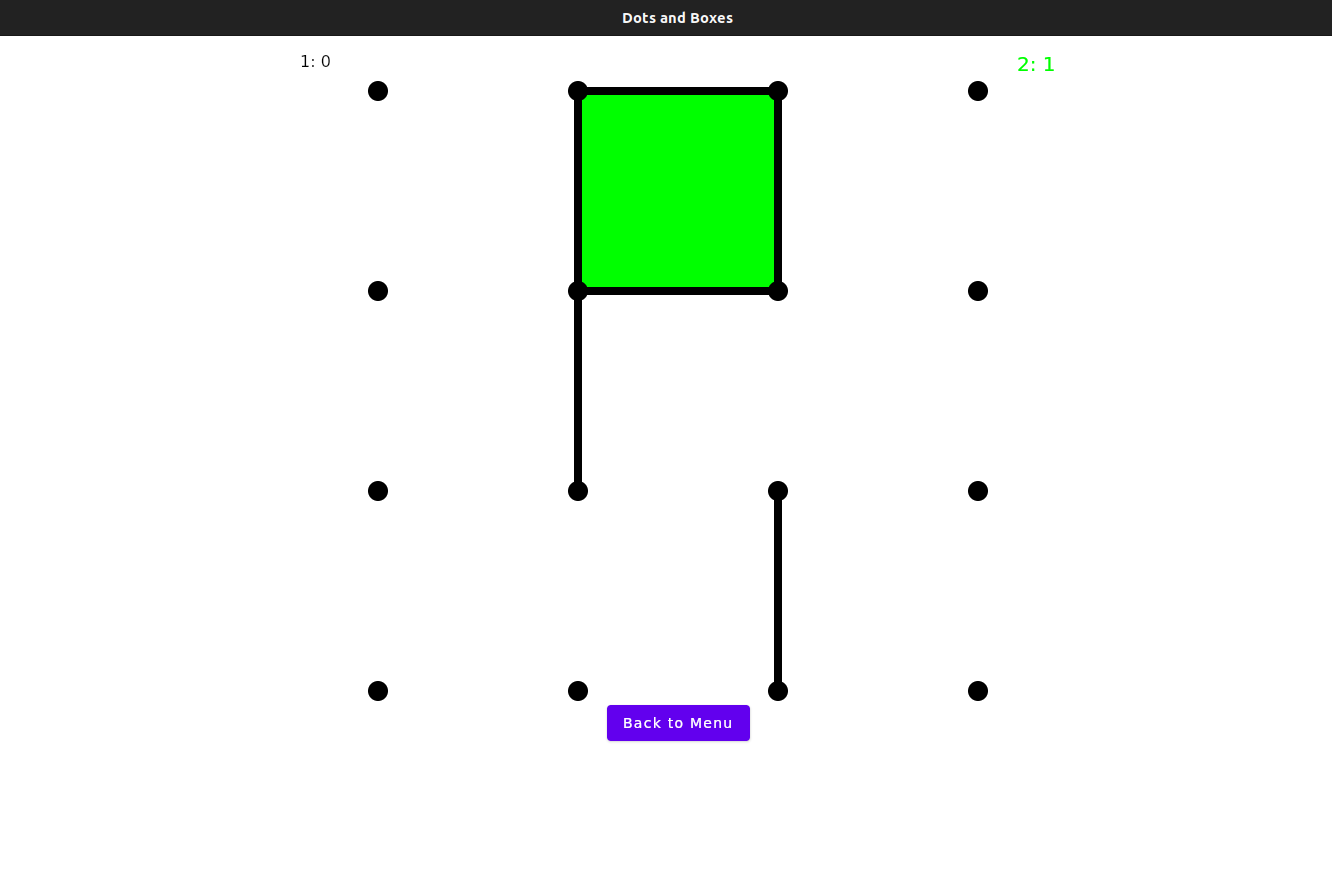
\includegraphics[width=0.8\textwidth]{gameBoard.png}
\end{center}
\end{frame}

\begin{frame}{Архитектура}
\begin{center}
\begin{tikzpicture}[
    node distance=1.2cm,
    block/.style={rectangle, draw, text width=4cm, align=center, minimum height=0.8cm, rounded corners}
]
\node[block, fill=gray!20] (ui) {UI (Compose Desktop)};
\node[block, below=of ui, fill=gray!20] (gc) {GameControl};
\node[block, below=of gc, fill=gray!20] (gl) {GameLogic};
\node[block, below=of gl, fill=gray!20] (b) {Data / IGameRule / IFieldShape};

\draw[->, thick] (ui) -- node[right] {вызывает} (gc);
\draw[->, thick] (gc) -- node[right] {использует} (gl);
\draw[->, thick] (gl) -- node[right] {использует} (b);
\end{tikzpicture}
\end{center}
\vspace{0.5cm}
\end{frame}

\begin{frame}{Архитектура}
\begin{center}
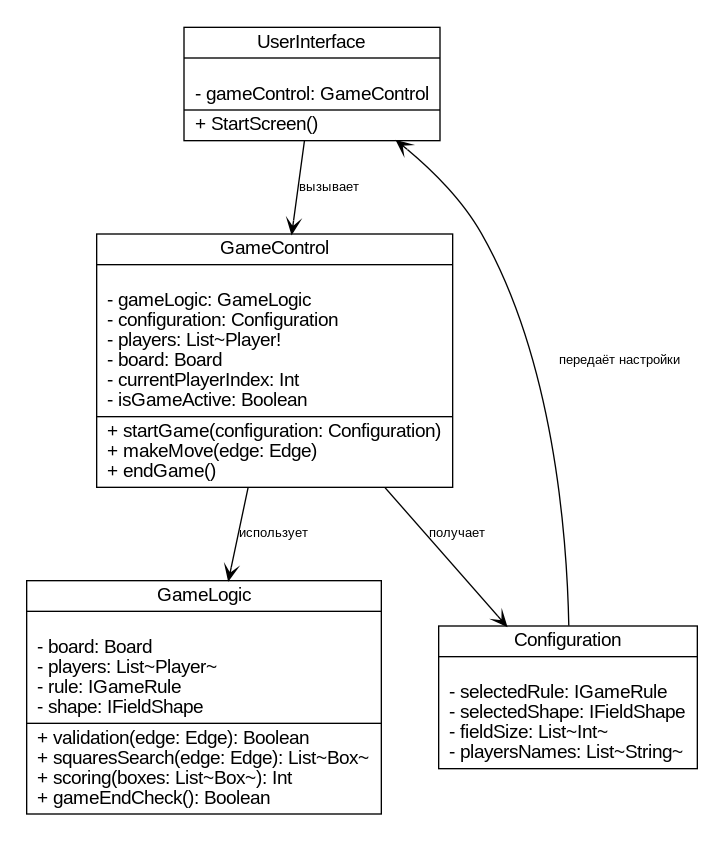
\includegraphics[width=0.4\textwidth]{first.png}
\end{center}
\end{frame}

\begin{frame}{Архитектура}
\begin{center}
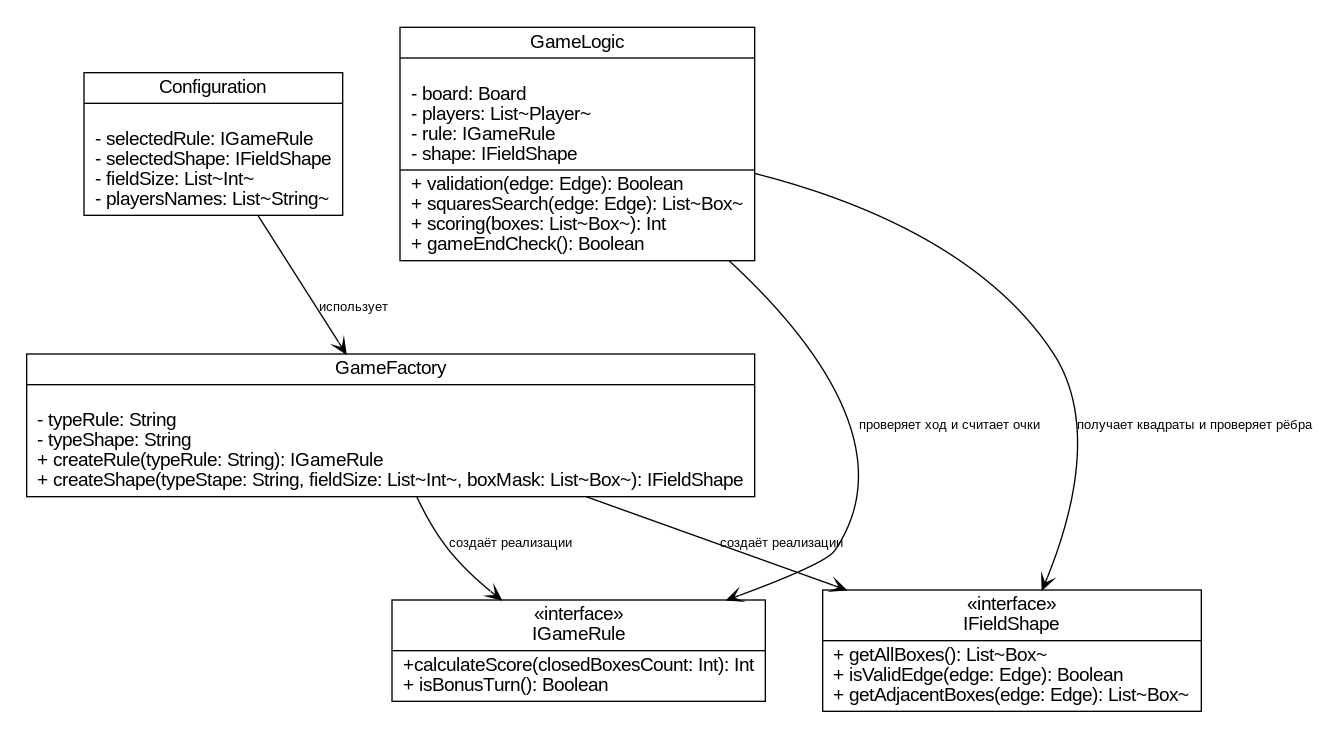
\includegraphics[width=0.8\textwidth]{second.png}
\end{center}
\end{frame}

\begin{frame}{Обработка хода}
\begin{center}
\begin{tikzpicture}[
    block/.style={rectangle, draw, text width=3cm, align=center, minimum height=1cm, font=\large},
    arrow/.style={->, thick}
]

\node[block, fill=gray!20] (ui) {UI Canvas};
\node[block, right=0.8cm of ui, fill=gray!20] (gc) {GameControl};
\node[block, right=0.8cm of gc, fill=gray!20] (gl) {GameLogic};
\node[block, right=0.8cm of gl, fill=gray!20] (b) {Board};

\draw[arrow] (ui) -- (gc);
\draw[arrow] (gc) -- (gl);
\draw[arrow] (gl) -- (b);

\draw[arrow, bend left] (b) to (gl);
\draw[arrow, bend left] (gl) to (gc);
\draw[arrow, bend left] (gc) to (ui);

\end{tikzpicture}
\end{center}
\end{frame}

\end{document}